\section{有向图}

\begin{definition}
	有向图去掉边的方向后得到的无向图为基础图. 无向图的每条边加上方向后得到的有向图为定向图.
\end{definition}
\begin{note}
	一个简单图有$2^{m(G)}$个定向图(\textcolor{red}{$n$阶完全图有$2^{\frac{n(n-1)}{2}}$个定向图}).
\end{note}

\begin{theorem}
	设$D=(V,E)$是一个有向图,则有
	\[
	\sum\limits_{v\in V}d^{+}(v)=\sum\limits_{v\in V}d^{-}(v)=m(D)
	\]
\end{theorem}

\begin{definition}
	设$D=(V, E)$是有向图,
\begin{enumerate}
	\item 若$D$的基础图是连通的,称$D$是弱连通图;
	\item 若$D$的中任意两点是单向连通的,称$D$是单向连通图;
	\item 若$D$的中任意两点是双向连通的,称$D$是强连通图;
\end{enumerate}
\end{definition}

\begin{note}
	\textcolor{red}{强连通一定单向连通,单向连通一定弱连通}.
\end{note}


\begin{example}
	在下图中,$D1, D2, D3$ 为弱连通图;$D1, D2$ 为单向连通图;$D1$ 为强连通图.
	\begin{figure}[H]
		\small
		\centering 
		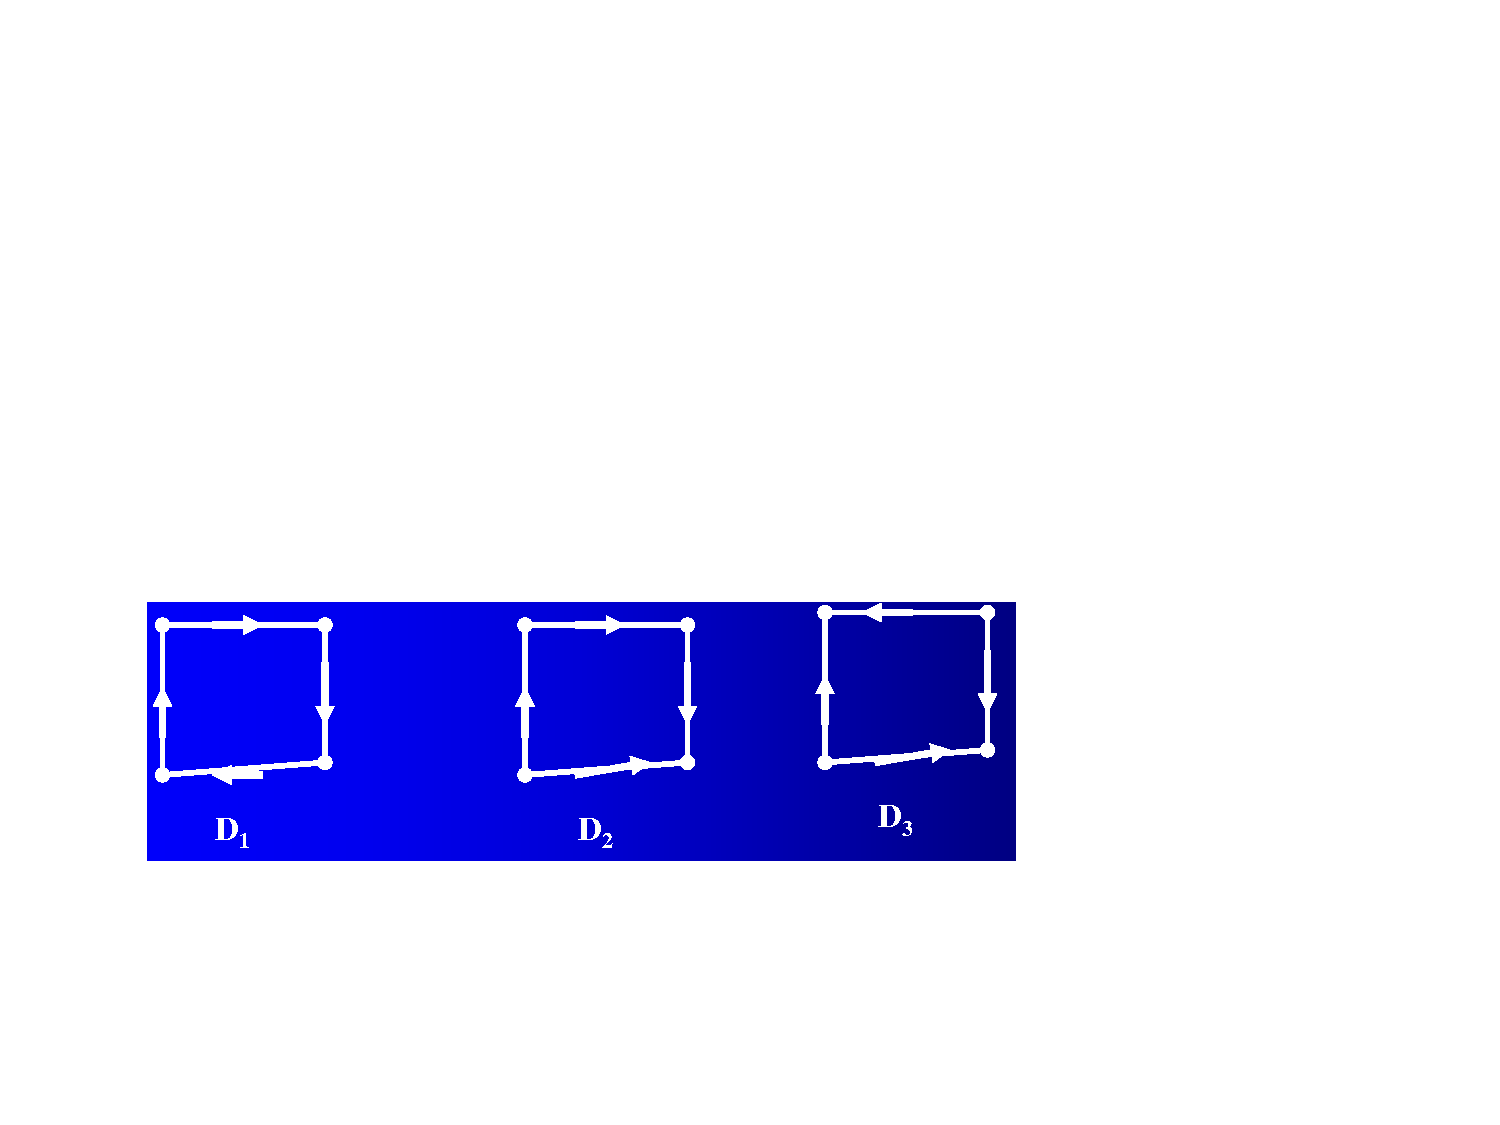
\includegraphics[scale=0.6]{image/CH9_liantong.pdf}  
		%\caption{信息包结构} 
		\label{figkk1ijjj}  
	\end{figure}
\end{example}

\begin{theorem}
有向图$D=(V,E)$是强连通的当且仅当 $D$ 中存在含有所有顶点的有向闭途
径.
\end{theorem}


\begin{definition}
	设 $D^{'}$ 是有向图 $D = (V, E)$ 的一个子图.如果 $D^{'}$ 是强连通的 (单向连通的、
	弱连通的),且 $D$ 中不存在真包含 $D^{'}$ 的子图是强连通的 (单向连通的、弱连通的),则称 $D^{'}$
	是 $D$ 的一个强连通分支 (单向连通分支、弱连通分支).
\end{definition}
\begin{example}
求下图$D$的强连通分支、单向连通分支.
	
\noindent {\bfseries\songti \textcolor{ecolor}{解:}} $D$的强连通分支$\{1\},\{5\},\{6\},\{2,3,4,7,8,9\}$. 由于$D$本身是单向连通的,故$D$的单向连通分支是$D$本身.	
		\begin{figure}[H]
		\small
		\centering 
		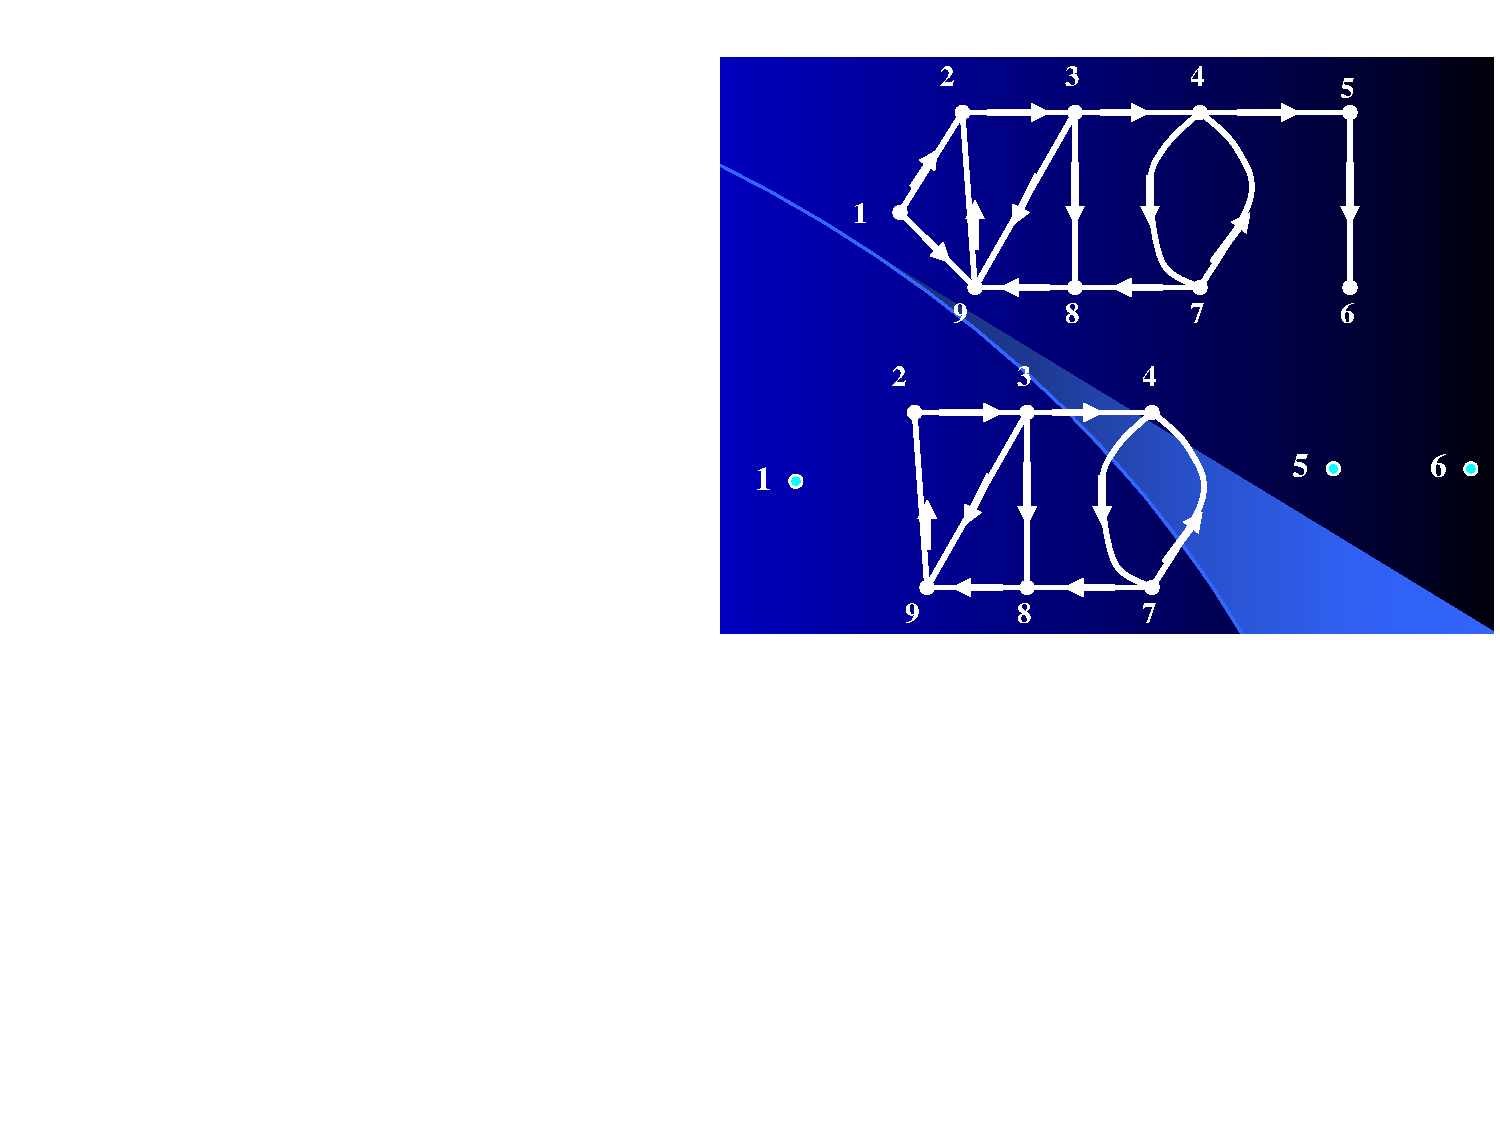
\includegraphics[scale=0.6]{image/CH9_qiangliantong.pdf}  
		%\caption{信息包结构} 
		\label{figkkk1ijjj}  
	\end{figure}
\end{example}


\begin{theorem}
有向图 $D = (V, E)$ 的每个点位于且仅位于$D$ 的一个强 (弱) 连通分支中.
\end{theorem}
\begin{note}
	\begin{enumerate}
		\item 强(弱)连通分支的并应该包含图中的任何一个点.
		\item 有向图 $D$ 的某个顶点$v$,可能处于$D$的不同单向连通分支中.
	\end{enumerate}
\end{note}


\begin{theorem}
	若 $G$ 是 2 边连通的,则 $G$ 存在强连通定向图..
\end{theorem}
